\vspace*{-0.2cm}

\section{Comparison Matrices}\label{sec:matrix}

\vspace*{-0.2cm}

We propose three detailed matrices which address the limits of WS3 identified in the previous section. 
The proposed matrices enable the comparison of technologies along a set of precise criteria to highlight their differences. 
These matrices extend the WS3 levels by adding new criteria which are used in practice (see section \ref{sec:insight}) and not linked to any WS3 levels.

\vspace*{-0.1cm}
\subsection{Insights from developers and architects}\label{sec:insight}

We interviewed 14 developers and architects from FABERNOVEL and clients on their experience with Semantic REST technologies. Raw results and the analysis are available online\footnote{\url{https://github.com/AntoineCheron/comparison-matrices-semantic-rest-api-techno}}. Our key findings are:
\begin{itemize}
 \item \textit{Selecting the technology:} 10 respondents have already built Semantic REST APIs: \textbf{30\%} spent more than two weeks selecting the technologies; \textbf{80\%} reported that the most difficult task was to understand the feature provided by each technology.
 \item \textit{Interchange Formats:} \textbf{6 out of 7} did not find a technology providing all required features (most often the missing features were the description of HTTP operations with their data model (3/8) and the Linked Data (2/8)). 
 \item \textit{Interface description languages:} All respondents said that none of them provide all required features (60\% said they lack the ability to describe links to other resources and business constraints; and 20\% of them would like to model the resources as finite state machines (FSM)).
 \item \textit{Frameworks:} 6 out of 7 reported that no framework offered the required feature. The missing features are related to the auto-documentation of the API, the automatic generation of link and a mechanism to model resources as FSM.
 \item \textit{Technology score:} The median value of the score is 2/5.
 %\item \textit{??:} have never built such APIs, none know the Semantic Web or Linked Data. One sees not interest in building HATEOAS APIs, another considers that the technologies are too difficult to find and the last one says that it is too time consuming.
\end{itemize}

These results emphasize the difficulties in selecting technologies associated to Semantic REST APIs. They also highlight that these technologies are not yet mature and give a rough idea of the missing features.

\subsection{Comparison Matrices Design Methodology}

The design of our comparison matrices follows a 5-step sequential process: \textit{(i)} \textbf{search} for candidate technologies, \textit{(ii)} \textbf{select} candidate technologies, \textit{(iii)} \textbf{read} carefully each candidate technology, \textit{(iv)} \textbf{elaborate fine grain criteria} to characterize and differentiate technologies, \textit{(v)} \textbf{verify} that the elaborated criteria highlighted the differences between technologies. We looped on step \textit{(iv)} and \textit{(v)} to avoid duplicating criteria or hiding important details.

The research of candidate technologies (step i) was done by:

\begin{enumerate}
    \item Searching Google and Google Scholar for Semantic REST Technologies using combinations of keywords from the set: ["web", "semantic", "restful", "rest", "service", "API", "interface", "description", "documentation", "language", "modeling", "hypermedia", "document", "format", "RDF", "data-interchange", "linked data", "hateoas", "rest api", "framework"];
    \item Searching Google Scholar for tools automating tasks from services description, using keywords: "matchmakers", "service composition", "service discovery", "rest service analysis", "automated mashups", we then selected papers and technologies from their references and the papers that cite those we selected;
    \item Searching the proceedings of ICWE and WS-REST. 
\end{enumerate}

We selected 81 papers, standards, articles and web pages (step ii) based on abstract or introduction. We selected documents that were specifications of interface description languages or models, frameworks supporting HATEOAS features, interchange formats that support RDF or HATEOAS features, comparisons between these technologies or tools leveraging them. Frameworks to build Semantic Web Services were excluded because they are based on triples, which are too far from the resource-oriented design of REST. We opened our research to technologies from the 1990s to today and retained those that are still available today.

As a next step, we read the specification of each chosen technology (step iii) and elaborated classification criteria (step iv). We included those of the H~Factor~\footnote{\url{http://amundsen.com/hypermedia/hfactor/}} which \textit{is a measurement of the level of hypermedia support and sophistication of a media-type}. Others were carefully designed to highlight differences between technologies, based on the core design of the technologies, the features they provide and the details of the WS3 maturity model. All the material is available online\footnote{\url{https://github.com/AntoineCheron/comparison-matrices-semantic-rest-api-techno}}.

As a final step (step v), we read the specifications again to verify results and validate that the selected criteria highlighted differences and commonalities well.

\paragraph{Popularity criteria}

We defined a popularity criteria to provide a rough idea of the community support and the likelihood of the technology to last in time. It respects the following rules: 
\begin{inparadesc}
    \item [0 -] Not enough to reach 1;
    \item [1 -] More than 100 questions on Stack Overflow AND (2500+ NPM weekly downloads OR 100+ maven usages);
    \item [2 -] More than 400 questions on Stack Overflow AND (500.000+ total downloads OR 15.000+ NPM weekly downloads OR 500+ maven usages).
\end{inparadesc}

\subsection{Interface Description Languages}

Interface Description Languages (IDLs) provide a vocabulary to document domain, functional and non-functional aspects of an API.
We identified 16 candidates that are classified according to 31 criteria in Fig~\ref{idl-matrix}. Among them, 4 are meta-models from conference papers \cite{10.1109/ICWS.2014.30} \cite{Rapido} \cite{Schreier:2011:MRA:1967428.1967434} \cite{10.1007/978-3-642-22233-7_24}. The 11 others are open-source projects or W3C recommendations.

In \cite{Rapido} authors present a tool to sketch CRUD or Hypermedia APIs. On the latter mode, users sketch the application using state-machines and then obtain a description in the HAL or Collection+JSON format.
\cite{Schreier:2011:MRA:1967428.1967434} models each resource type as a finite-state-machine with deterministic transitions and conditions to inform about the availability of transitions. However, they are not modeled in more details, which make them not machine-interpretable.
In~\cite{10.1007/978-3-642-22233-7_24}, authors propose to model systems as non-deterministic state machines. This method thus makes software agents unable to discover the set of messages to exchange in order to make an operation available.
Haupt et al.~\cite{10.1109/ICWS.2014.30} propose a multi-layered model that separates the domain model from the URI model. However, resources have a fixed model, which does not allow them to have a data model adapted to each state.

It is important to note than when \textbf{IDLs and interchange formats} are both \textbf{compatible with RDF}, they can be combined to form a file format usable as data-interchange format and IDL. This has great benefits to lower the overall complexity and increase the evolvability of the system.

% FIGURE OF THE IDL CLASSIFICATION
\begin{figure*}[!ht]
\caption{Interface Description Languages Comparison Matrix}
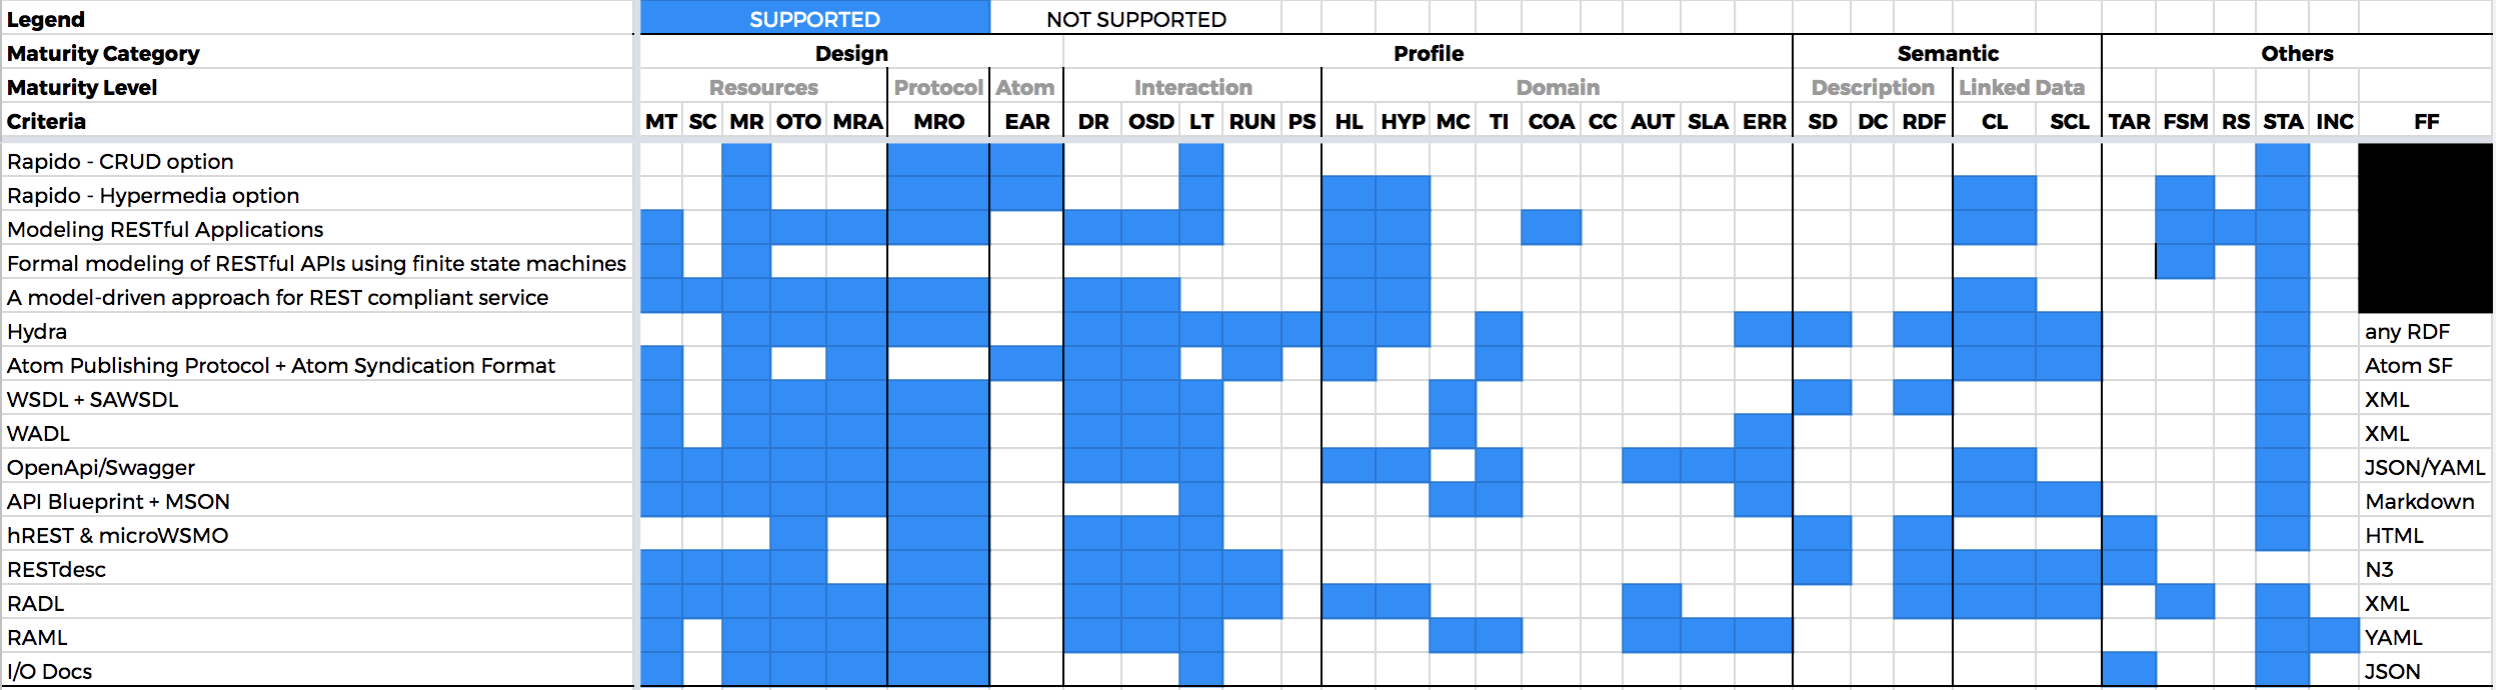
\includegraphics[width=1\textwidth]{figures/IDL.png}
\label{idl-matrix}
\vspace{-1.2cm}
\end{figure*}

\subsubsection*{Synthesis}

First, the matrix highlights the fact that most technologies help with building mature systems on the \textit{design} dimension and \textit{interaction profile} level of the \textit{profile} dimension, D3-P1 following the WS3 categories.
On the other hand on the \textit{semantic} dimension, we notice that 5/16 technologies support the use of RDF vocabulary, which allows to build Linked Data APIs. As a reminder, this is required to reach full Semantic REST compliance.
Moreover, by supporting the use of RDF vocabulary, IDLs can be enriched to reach a higher level of maturity.

Among the technologies, four can be distinguished by the number of criteria they meet: Hydra (18), RADL (18), OpenAPI (17) and RESTdesc (17).
OpenAPI is the only one that has no support for RDF. Thus, it helps in building systems up to D3-P2-S0 on the WS3 scale.
On the other hand, Hydra, RADL and RESTdesc support the use of RDF vocabulary, which makes these technologies better suited to build systems that are mature on the semantic dimension.

\textit{Towards HATEOAS APIs}
From the matrix, we notice that most technologies target the documentation of the API in a single, non-splittable file. Hence, they are not suited to provide hypermedia controls at runtime.

On the other hand, only one approach, \cite{Schreier:2011:MRA:1967428.1967434}, supports the description of the conditions that determine the availability of a link, and none makes this meta-data machine-interpretable. This makes software agents unable to find a way to make an operation available when it is not.

\textit{Towards better-documented APIs}
Only four technologies support the description of business constraints which lowers coupling and improves user experience, e.g., with the automatic generation of forms with client-side validation.

Finally, we note that most scientific publications recommend the modeling of RESTful systems with state-machines whereas open-sourced or W3C IDL authors don't consider this design method. And yet, the use of deterministic state-machines eases the determination of the available operations of a resource.

\subsection{Data-interchange formats}

Data-interchange formats provide a data-structure, a vocabulary and a layout to represent a resource and its meta-data at runtime. When the API does not need to send meta-data, JSON and XML are the two widely used formats in the industry.

On the other side, when the system to be built have to support a hypermedia interchange format, none is considered as a standard today. We selected 11 candidate technologies, which are classified in Fig.~\ref{interchange-formats-matrix} according to 24 criteria. JSON is included for comparison purposes.

% FIGURE OF THE INTERCHANGE FORMATS CLASSIFICATION
\begin{figure*}[!ht]
\caption{Data-interchange Formats Comparison Matrix}
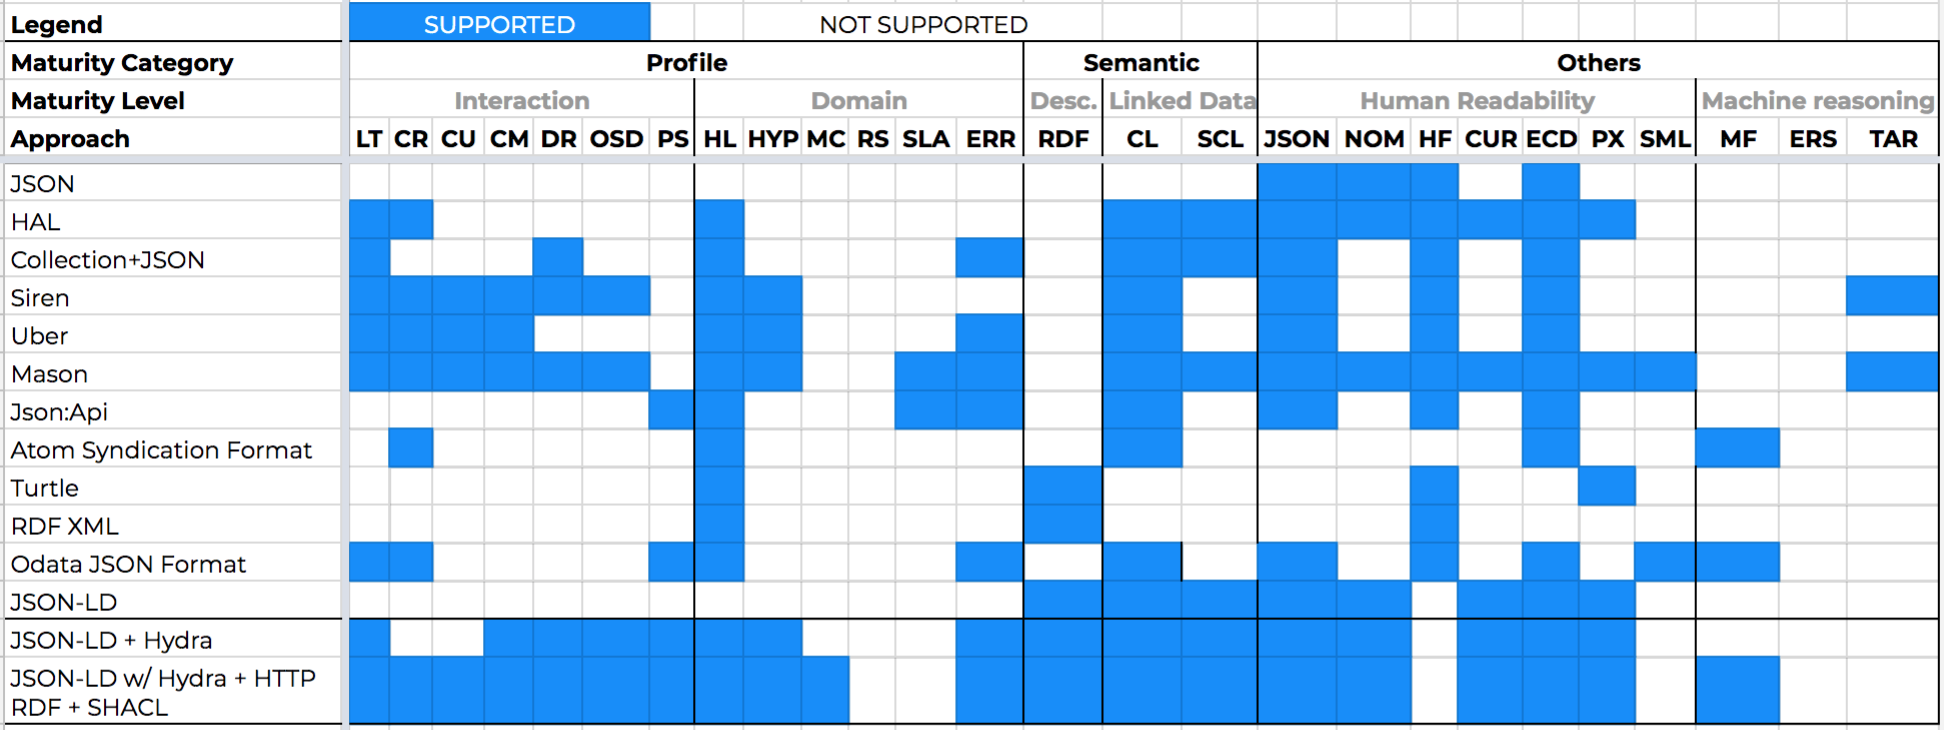
\includegraphics[width=1\textwidth]{figures/DIF.png}
\label{interchange-formats-matrix}
\vspace*{-0.7cm}
\end{figure*}

\subsubsection*{Synthesis}
First, from this matrix, we notice that formats can be differentiated based on their compatibility with RDF. Indeed, RDF formats (Turtle, RDF XML and JSON-LD) can be enriched with RDF vocabularies. This is why they propose very few features by default. To depict what is achievable by combining vocabularies with a RDF format, we selected two vocabularies: Hydra and SHACL, a RDF schema validation vocabulary, that we combined with JSON-LD and evaluated them. As a result, they match 12 more criteria than JSON-LD alone.
From this, we infer that combining RDF formats with vocabularies allow building mature Semantic REST systems. However, this requires additional effort to find relevant vocabularies.
On the other hand, non-RDF formats help building systems that can be mature on the \textit{profile} dimension but not on the \textit{semantic} dimension.

Furthermore, the matrix shows that no format supports the description of constraints despite the fact that it can be leveraged to reduce coupling and improve the user-experience.

Finally, it highlights that no format advertise the state of the resource even though most scientific approaches we found describe REST APIs as state-machines.

\subsection{Implementation Frameworks}

Implementation frameworks are software libraries that guide developers through the implementation of Web APIs. We limit the comparison to frameworks that claim to support HATEOAS. We identified six frameworks that do so. Frameworks to build Semantic Web Services are excluded because their triple-centric approach differs too much from REST.

Among the selected papers, in \cite{salvadori2014framework} authors propose \textit{Hypermedia Web API Support}, a Java framework based on JAX-RS 2.0 that offers annotations to semantically describe REST APIs. The end result is the description of the whole API in a JSON-LD document enriched with the Hydra vocabulary. Unfortunately, the framework is not available in Maven Central. In \cite{parastatidis2010role} Parastatidis et al. present \textit{Restfulie}, a framework that uses resources, state transitions and content-negotiation as its core building blocks. We found 4 other frameworks that support HATEOAS features. They are all classified in Fig.~\ref{frameworks-matrix} according to 23 criteria.

% FIGURE OF THE IMPLEMENTATION FRAMEWORKS CLASSIFICATION
\begin{figure*}[!ht]
\caption{Implementation Frameworks Comparison Matrix}
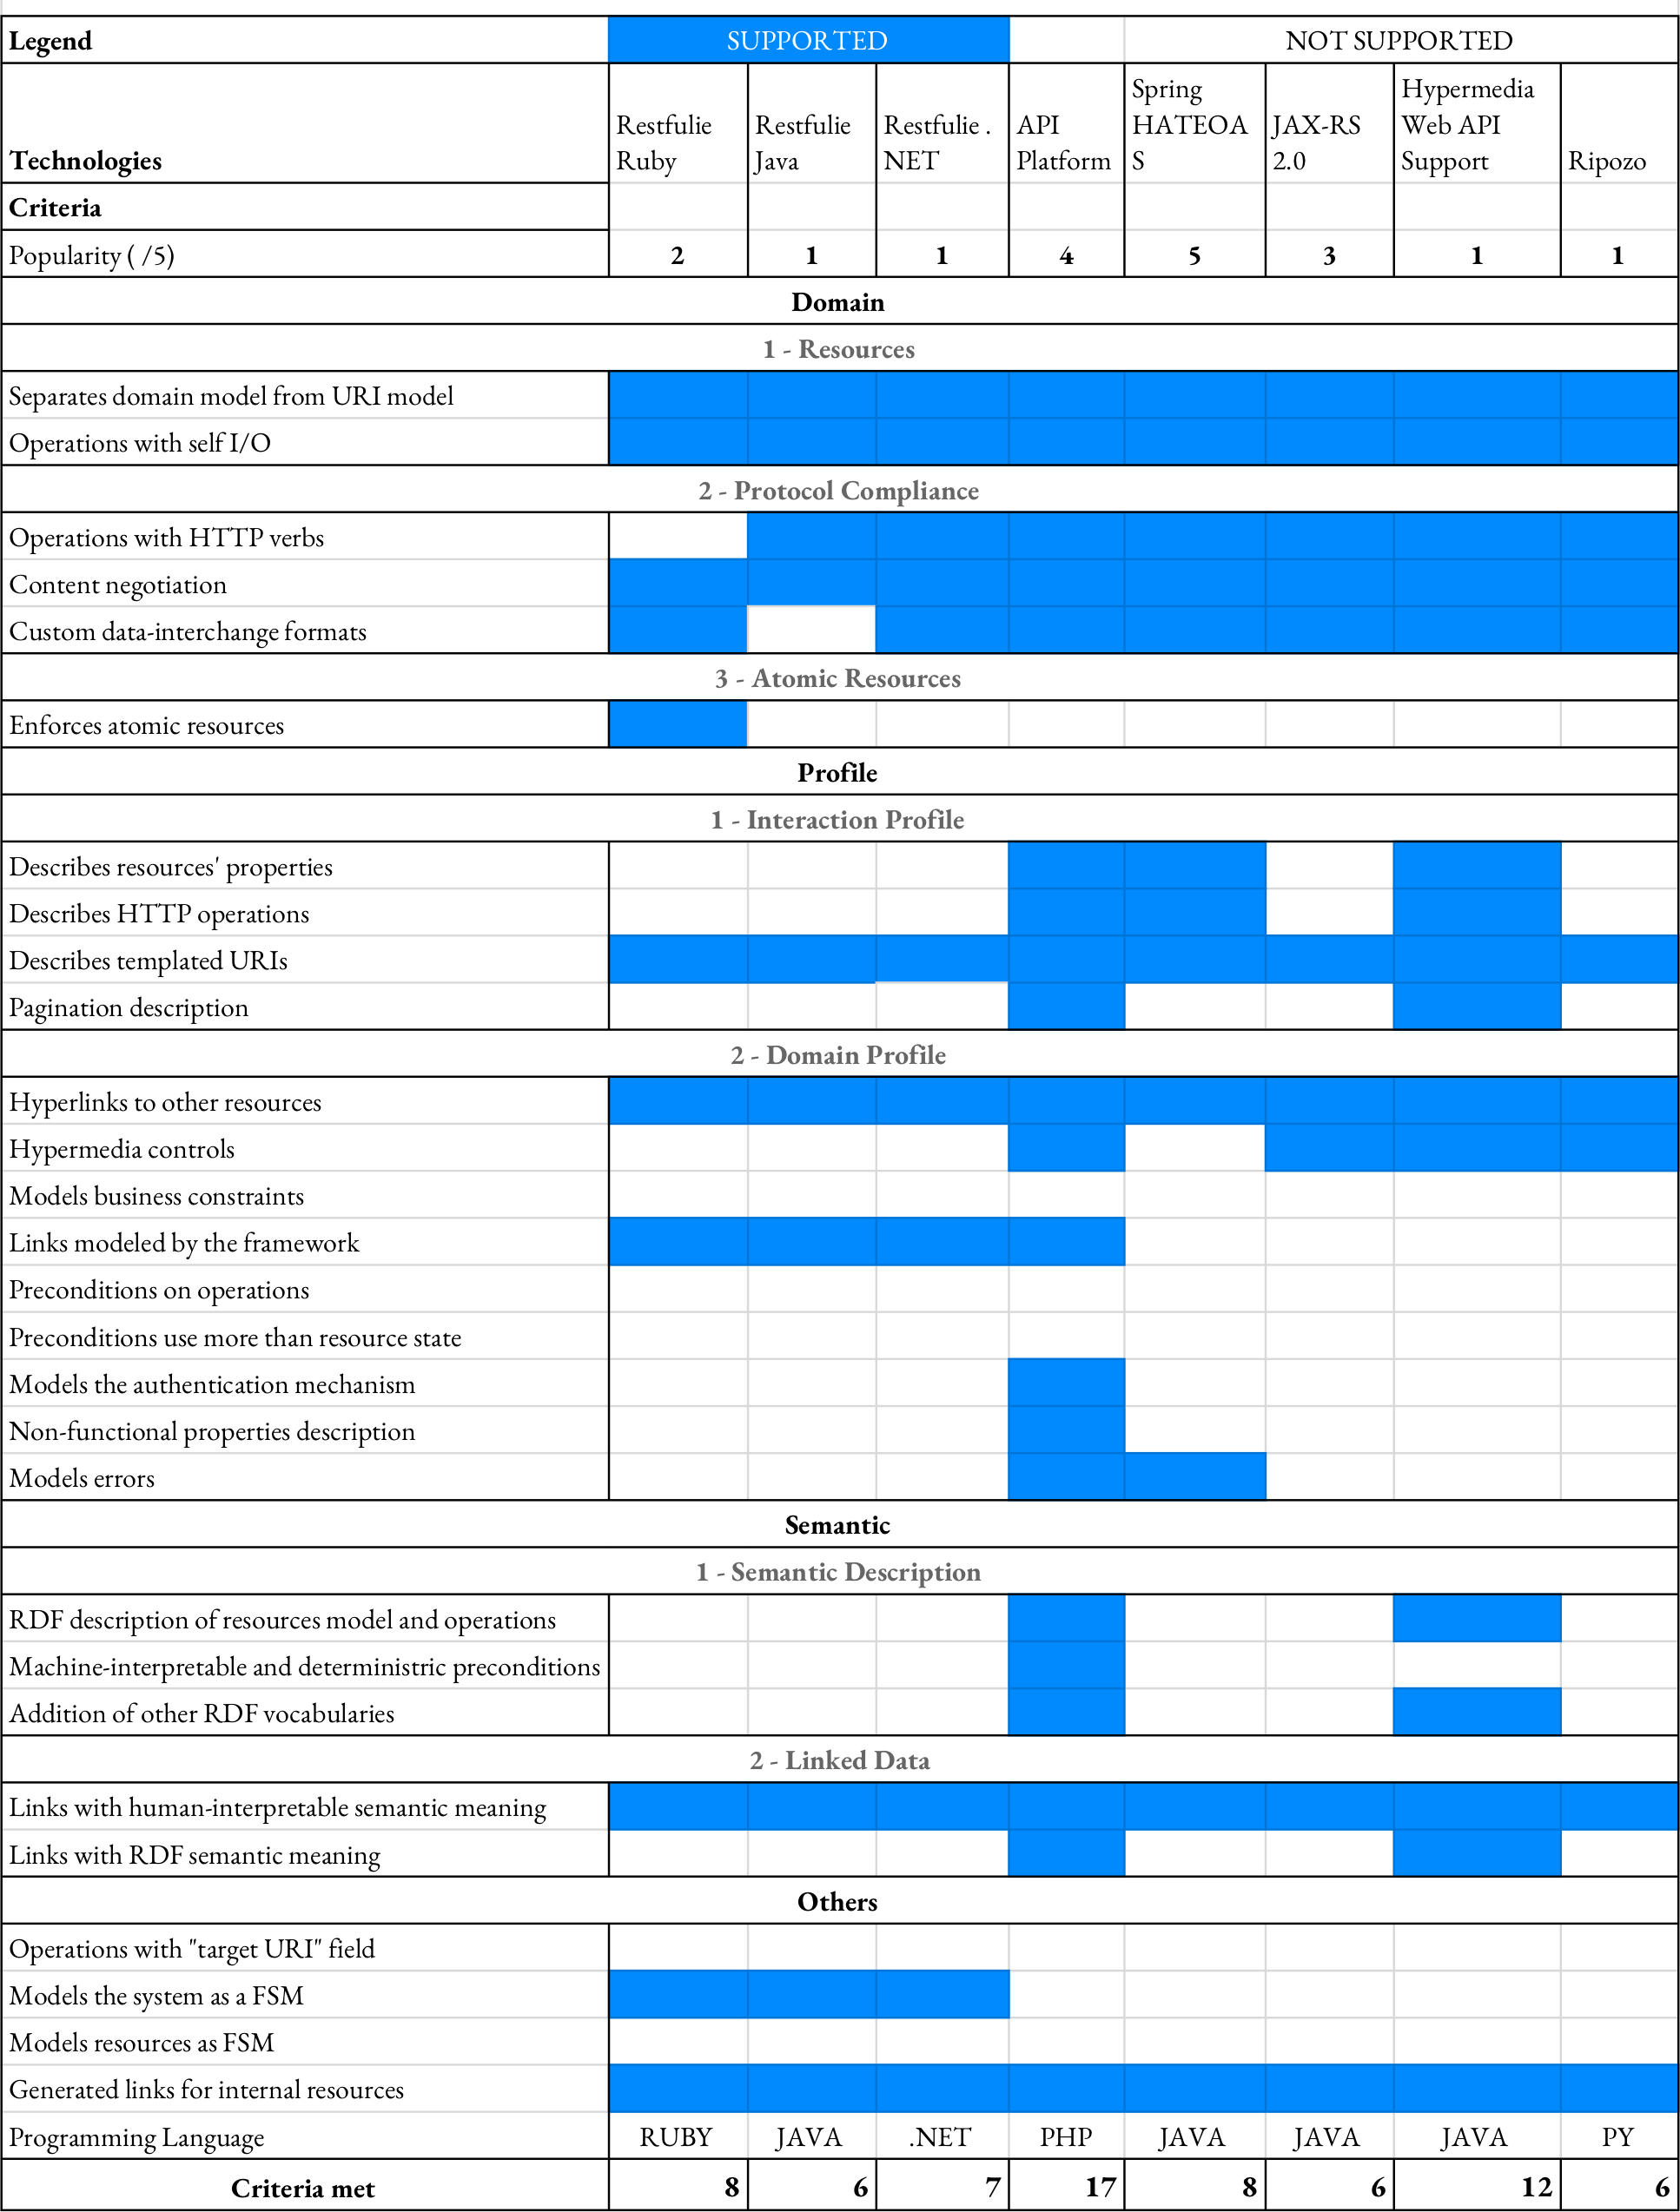
\includegraphics[width=1\textwidth]{figures/frameworks.png}
\label{frameworks-matrix}
\end{figure*}

\subsubsection*{Synthesis}
Despite the fact that only one framework enforces the \textit{Atomic Resources} constraint, all frameworks allow to reach the highest level of maturity on the \textit{design} dimension easily. This is because supporting the \textit{Atomic Resources} constraint only requires developers to use the data model of the resource as the input of write operations and as the output of read operations.\\
We notice that only \textit{API Platform} and \textit{Restfulie} offer a mechanism to model relations between resources from which links are automatically generated, instead of adding them programmatically in the response, thus increasing maintainability.\\
Otherwise, most frameworks do not ease the semantic and domain description of APIs. To us, this is the biggest challenge framework designers should tackle.\\
Last, as for IDLs, most frameworks creators do not provide mechanisms to describe resources as state machines, thus not taking advantage of its benefits.
